\documentclass[12pt]{article}
\usepackage{sectsty}
\usepackage{dirtytalk}
\usepackage{graphicx}

\sectionfont{\large}
\subsectionfont{\large}
\renewcommand{\thesubsection}{\thesection.\alph{subsection}}


\title{\vspace{-2cm}CMPSCI 590F Digital Forensics Assignment 12: THD, Phone Forensics, TRIM}
\author{Vinitra Ramasubramaniam}
\begin{document}
\maketitle
\section{Define the \say{Trojan Horse defense} in terms of \say{actus reus} and \say{mens rea}.}
\say{For the Trojan Horse Defense, the defendant can claim that he may have committed the actions (actus reus) of the crime, but done so unknowingly (mens reus). Actus reus, refers to the act of committing the crime while mens reus refers to the intention or knowledge of the crime.}
\section{List two methods of countering the Trojan Horse defense that can be performed by law enforcement during the execution of a search warrant and/or interview.}
\say{First, the factual basis of the defense can be negated. The law enforcement could thoroughly examine the drives, looking for malware. If found, it should be determined if its capabilities permit the alleged crime. If not, one should look for evidence of wiping or wiping tools.\\
Second, law enforcement could seek confessions in interrogation or before. As noted by Brenner et al., suspects often confess, and these confessions are binding (assuming the suspect has been Mirandized appropriately). Some questions that can be asked that rule out (or make more difficult) the \say{Trojan Horse Defense} or the \say{Some Other Dude Did It defense} are \say{Who else has access to the computer in question?} \say{Do you use antivirus programs?} etc.}
\section{Garfinkel et al.'s article on small block forensics is motivated by four main reasons. They state at the start of the article, \say{there is a growing need for automated techniques and tools that operate on bulk data, and specifically on bulk data at the block level.} What are these reasons?}
\say{The four reasons that motivate Garfinkel et al.'s article on small block forensics are:
\begin{enumerate}
\item File systems and files may not be recoverable due to damage, media failure, partial overwriting, or the use of an unknown file system.
\item There may be insufficient time to read the entire file system, or a need to process data in parallel.
\item File contents may be encrypted.
\item The tree structure of file systems makes it hard to parallelize many types of forensic operations.}
\end{enumerate}
\section{The \say{small block forensics} approach proposed by Garfinkel et al. includes the use of sampling from a drive to find files already known to be of interest. Suppose you've recently acquired 160TiB (that is, $160 * 2^40$ bytes) of data, and you are looking for any portion of 512GiB ($512 * 2^30$ bytes) of files that you know to be of interest. How many 4096 byte samples (uniform, at random, without replacement) would you expect to have to take from the drive such that the probability of failing to find even one of the files of interest is less than 0.01\% (that is, p $<$ 0.0001)? Make the simplifying assumption that all files are located at 4096 byte offsets.}
\begin{equation*}
\textrm{Total size of disk in bytes} = 160 * 2^{40}
\end{equation*}\\
\begin{equation*}
\textrm{Total size of interesting file in bytes} = 512 * 2^{30}
\end{equation*}\\
\begin{equation*}
\textrm{Size of offset in bytes} = 4096 = 2^{12}
\end{equation*}\\
Therefore, the total number of blocks possibly containing an interesting file is given by:\\
\begin{equation*}
\begin{split}
\( \displaystyle \frac{160 * 2^{40} - 512 * 2^{30}}{2^{12}}\) = 160 * 2^{28} - 512 * 2^{18}} \\= 2^{18}(160 * 2^{10} - 512) = 2^{18}(160 * 1024 - 512) = 2^{18}(163840 - 512)\\ = 163328 * 2^{18}
\end{split}
\end{equation*}\\
Let us say $n = 163328 * 2^{18}$
The probability that we find the interesting file in the first block is:\\
\begin{equation*}
\( \displaystyle \frac{1}{n}\) = \( \displaystyle \frac{1}{163328 * 2^{18}}\)
\end{equation*}\\
The probability that we find one interesting file in the second block is the probability that we don't find the interesting file in the first block and probability that we find the interesting file in the second block:\\
\begin{equation*}
(1- \( \displaystyle \frac{1}{n}\)) * \( \displaystyle \frac{1}{n-1}\) = \( \displaystyle \frac{n-1}{n}\) * \( \displaystyle \frac{1}{n-1}\) = \( \displaystyle \frac{1}{n}\) = \( \displaystyle \frac{1}{163328 * 2^{18}}\)
\end{equation*}\\
Similarly, the probability that we find the interesting file at each block, up to n is:\\
\begin{equation*}
= \( \displaystyle \frac{1}{n}\) = \( \displaystyle \frac{1}{163328 * 2^{18}}\)
\end{equation*}\\
Let us say $T$ is the number of samples. Considering, the samples are uniform, random and without replacement, the minimum number of samples required such that the probability of failing to find at least one interesting file $< 0.0001$ is:\\
\begin{equation*}
\begin{split}
\implies T* \( \displaystyle \frac{1}{n}\) \ge 0.0001\\ \implies T \ge \( \displaystyle \frac{1}{n}\) * 0.0001\\
\implies T \ge \( \displaystyle \frac{1}{163328 * 2^{18}}\) * 0.0001\\
\implies T \ge 163228 * 26.2144\\
\implies T \ge 4278924.08
\end{split}
\end{equation*}\\
Thus, the minimum number of 4096 bytes samples one is expectd to take from the drive such that the probability of failing to find even one of the files of interest is less than 0.01\% (that is, p $<$ 0.0001) is 4278925.
\section{Describe the basic use of block hash filtering in the Walls et al. article on DEC0DE. What are the specific steps that are taken?}
DEC0DE's block hash filtering component (BHF) is based on the notion that long identical byte sequences
found on different phones are unnecessary for triage. That is, such sequences are unlikely to contain useful information for investigators.\\
\begin{figure}[h]
\centering
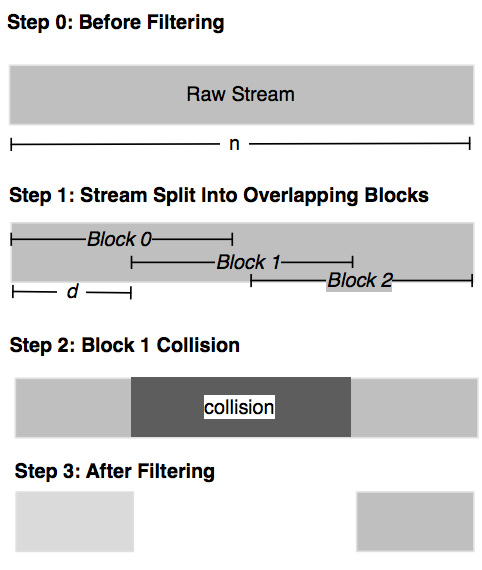
\includegraphics[width=0.5\textwidth]{bhf.png}
\caption{Block Hash Filtering}
\label{fig:bhf}
\end{figure}
Block hash filtering takes a stream of $n$ bytes and creates a series of overlapping blocks of length $b$. The start of each block differs by $d \le b$ bytes. Any collision of the hash of a block with a block on another phone (or the same phone) is filtered out. This is illustrated in Figure~\ref{fig:bhf}
\section{Explain the purpose of TRIM for solid-state drives; also explain the performance implications of not supporting TRIM.}
\say{Flash memory of the type we see in SDDs is built atop floating gate metal-oxide-semiconductor field-effect transistors. These are programmable transistors that act like NAND gates (readable). They start in one state and can be \say{set} (written) to another, or \say{reset} (erased). We can read. We can write, once. But to re-write, a whole \say{block} of NAND gates must be re-set to their base state first. Notably, erasing is the slowest operation by far. (Typically by at least one order of magnitude.) SSD controllers then have a choice. They can allow overwrites of a given \say{sector} by erasing then writing. Or they can dynamically map sectors to arbitrary, ready-to-write (already erased) locations in their flash arrays. The \say{empty} but not erased sectors can then be erased by the drive controller when the drive is otherwise idle. The former strategy leads to lackluster performance, since writes are then only as fast as erasures. The latter strategy is the TRIM command.\\
TRIM is, in short, a command that the disk driver in the OS can send to SDD-based disk controllers. TRIMming a sector tells the SDD that the sector in question can be erased - it is not being used to store data any more). The better integrated the OS/hardware/etc, the more likely it is to work, as the OS, driver, interface, and controller must all correctly implement TRIM for the command to be issued. Blocks scheduled for TRIMming will be erased by the controller even if the device is behind a write blocker.}
\section{Microsoft supports TRIM for NTFS filesystems on recent versions of Windows. Explain why the recoverability of a very small file in particular (for example, a file storing a 64 byte private key) would or would not be affected the use of TRIM on an SSD drive.}
Most hard drives used in Windows systems are using NTFS as their file system. NTFS stores information about the files and directories in the Master File Table (MFT). MFT contains information about all files and directories listed in the file system. In other words, each file or directory has at least one record in MFT. In terms of computer forensics, one particular feature of MFT is of great interest. Unique to NTFS is the ability to store small files directly in the file system. The entire content of a small file can be stored as an attribute inside an MFT record, greatly improving reading performance and decreasing wasted disk space (\say{slack} space). As a result, small files being deleted are not going anywhere. Their entire content continues residing in the file system. The MFT records are not emptied, and are not affected by the TRIM command. This in turn allows investigators recovering such resident files by carving the file system. The maximum size of a resident file cannot exceed 982 bytes which can easily accommodate a file storing a 64 byte private key.
\end{document}